\documentclass{article}
\usepackage{cite}
\usepackage{graphicx}
\usepackage{amsmath}
\newcommand\norm[1]{\left\lVert#1\right\rVert}
\DeclareMathOperator*{\argmin}{arg\,min}

\setlength{\parindent}{0cm}
\setlength{\parskip}{0.25cm}

\begin{document}
\author{Max Horowitz-Gelb}
\title{Active Learning For DBSI: DNA Binding Site Identifier }
\maketitle

\section*{Abstract}
DBSI is a structure based method for predicting the positions of protein interaction sites associated with DNA binding \cite{dbsi}. Here I present a method for applying active learning to the training of DBSI. This method optimizes the training of DBSI in a way that considers the batch style form of labelled data collection necessary when creating a training set. This method shows slight improvements in efficiency in comparison to naive methods. 
\section*{Introduction}
For area under an ROC curve, DBSI has been shown to achieve $~88\%$, a high degree of separability. The score was achieved by training DBSI on a set of 263 unique proteins. The model as a result of this training is now accessible to anyone on a public server \cite{dbsi_server}. The quality of this model could be improved further by training with more labelled data. But to collect more data practically we need to address practical issues.
\subsection*{Necessity for Active Learning}
Unlike learning on data generated from sensors or internet activity, aquiring labelled data for DBSI requires considerable time and energy. Experiments must be done to probe each protein for interaction sites. Much of this labelled data can be generated computationally from protein-DNA complex databases as described in \cite{displar}.
But for many complexes, particularly for Protein-RNA complexes, there is still no data. Even for complexes that do exist in databases, there are thousands of them and one cannot reasonably extract all of them. 

Because of these issues one needs a strategy for selecting data they would like labelled. There is a need for a method that can find data that has the most potential for being informative, without knowing its label. This is exactly what active learning methods try to do. Active learning is a process in which a machine learning model iteratively retrains itself as new labelled data points come in. The active learner is responsible for requesting, also known as querying, the labels of training data it thinks will be most informative to the current trained model.  

\subsection*{Neccessity for batch style active learning}
Due to the way training data for DBSI is aquired, standard active learning methods are not appropriate. This is because each training point given to DBSI corresponds to one residue in a protein. Therefore each protein that is probed will give hundreds of new training points. Because of this we must query training points in batches as opposed to querying individual residues. This puts us in a unique situation where the batch with the most informative set training points as a whole may be different than the batch containing the one individually most informative training point. To address this issue I use a active learning querying method which scores batches rather than individual points in order to select the next query protein.

     
\section*{Methods}
DBSI uses a support vector machine to classify residues. Such machine learning model has geometric properties that make applying active learning quite intuitive. 

\subsection*{Non Batch-Style Active Learning}
Let us consider a standard binary classifier SVM as DBSI uses.
Then we have a set of $n$ training examples
$
\{(x_1,y_1),...,(x_n, y_n)\} \subset (X \times \{-1,1\})^n
$ where $X$ denotes our input space. 


 as shown in \cite{svm}, our decision function can be described by its training examples,
\[
g(x) = \sum_{i=1}^{n} \alpha_i k( x_i, x)
\]
and classifcation is simply the sign,
\[
	f(x) = sign(g(x))
\]
Where $x_i$ is the set of support vectors,
$x$ is our vector we want to classify, $\alpha_i$ selects our support vectors, and $k$ is our kernel function.

As shown in \cite{active_learning}, if our kernel $k$ satisfies Mercer's condition, then there exists a feature space $F$ and a map $\phi$ from $X$ to $F$, such that $k(x,x') = \langle \phi(x) , \phi(x') \rangle$, and we may rewrite our above equation as
 
\[
f(x) = sign(\langle w_{svm}, \phi(x) \rangle)
\]
\[
w_{svm} = \sum_{i=1}^n \alpha_i \phi(x_i)
\]
where $w_{svm}$ is the normal vector of our hyperplane in feature space. 

If we assume our training data is linearly separable in $F$ then there is exists a non-empty set
\[
V = \{w \in F | y_i \langle w, \phi(x_i) \rangle > 0 \text{ for } i = 1, ...,n \text{ and} \norm{w} = 1
\]
which we call our version space \cite{version_space}.

Now let $Q \in X^m$ be our query pool that our active learner has access to and
$l : X \rightarrow \{-1,1\}$ be a function giving the correct label of an instance of our query pool.

Then at each step our active learner removes one instance $x_{n+1}$ from $Q$ and then adds it to our training set resulting in a new training set
\[
\{(x_1, y_1),...,(x_n,y_n)\}\cup\{(x_{n+1}, l(x_{n+1})\}
\]


For an efficient learning we want an active learner who most rapidly decays the cardinality of $V$ as it adds individual examples to our training set. As shown in \cite{active_learning} we can guarantee a high decay in $|V|$ by querying the instance closest to the hyperplane in feature space. So at each active learning query step we query
\[
x_{n+1} = \argmin_{x' \in Q} |g(x')|
\]

For active learning in a setting where we query one instance at a time, this works fairly well, but this is not the case in batch style active learning. 

\subsection*{Batch-Style Active Learning}

Batch-style active learning is very similar to standard active learning except now we remove multiple instances from the query pool at the same time. So for a batch size of $p$ we remove a query batch
$B \in X^p | B \subset Q$.


Intuitively one might extrapolate from the single instance case of active learning and select $B$ to be the $p$ instances in $Q$ closest to the hyperplane. As shown in \cite{active_learning}, this turns out to be a naive approach since the points may be close and contain redundant information. A better solution is one that not only considers distance from the hyperplane but also diversity of the points. Diversity in this case is measured using the angle between the induced hyperplanes of two instances. The induced hyperplane $h$ of an instance $x$ is the hyperplane whose normal vector is orthogonal to $\phi(x)$. From \cite{active_learning} we can calculate angles between the induced hyperplanes of two instances $x_1$ and $x_2$ as
\[
|cos(\angle(h_1, h_2))| = \frac{|k(x_1,x_2)|}{\sqrt{k(x_1,x_1)k(x_2, x_2)}}
\]

Then we can score each instance in $Q$ for its redundancy to in comparison to all other instances as
\[
r(x) = \max_{x' \in Q, x' \neq x} \frac{|k(x,x')|}{\sqrt{k(x,x)k(x', x')}}
\]

Then for each instance $x$ in the query pool we give it a score
\[
s(x) = \lambda |g(x)| + (1- \lambda) r(x)
\]
where $\lambda$ is a weight parameter between $0$ and $1$ which controls how much priority we give to each sub-score. 

Then for as described in \cite{active_learning}, we set our query batch $B$ equal to the $p$ instances in $Q$ with lowest scores or
\[
B = \argmin_{b \in X^p, b \subset Q} \sum_{x \in b} s(x)
\]

\subsection*{Active Learning Used for DBSI}
This batch-style method described above is slightly incompatible with DBSI since in \cite{active_learning} this method allows the active learner to create a query batch of any of the instances in the query pool. In the setting of DBSI, the batches are already predefined. Each instance is a member of a batch corresponding to the protein from which the instance came from. This is not a huge incompatibility. It only means that now the batches are pre-set and the active learner must score these batches instead of the individual instances. To do this, each batch is given a score
\[
s_{batch}(B) = \sum_{x \in I(B)} \lambda * (1- |g(x)|) + (1-\lambda) * (1 - r(x))
\]
where $I(B)$ is the set of instances $\{x \in B : |g(x)| < 1\}$. Then at each query step we simply select the predefined batch $B$ that maximizes $s_{batch}(B)$.

\section*{Results}
\subsection*{Evaluation}
To evaluate the active learning method described above, the training set of 263 proteins from \cite{dbsi_server} was divided into three sets. One was an initial training set of 100 proteins, one a query pool of 123 proteins and one test set of 40 proteins. Due to data in \cite{dbsi_server} being heavily modified over time, information of corresponding protein for each training instance was lost. To simulate having this information, all the training instances were divided equally into different batches, each of approximately 200 instances. Each batch simulated the existence of one protein. 

For evaluation the same learning parameters were used as in \cite{dbsi_server}, the rbf kernel with $\gamma = 0.0008$. Then the SVM was fitted to the initial training set. Then the active learning method was applied for 123 steps until it had queried all the proteins in the query pool set. After each query step the new fitted SVM was evaluated against the test set using area under the ROC curve. 

In order to have a baseline for comparison, this same process was run with a random query method instead of the active learning method. As its name implies this random query method queried proteins from the query pool set completely randomly without regard for the contents of each protein batch. 
\subsection*{Performance}

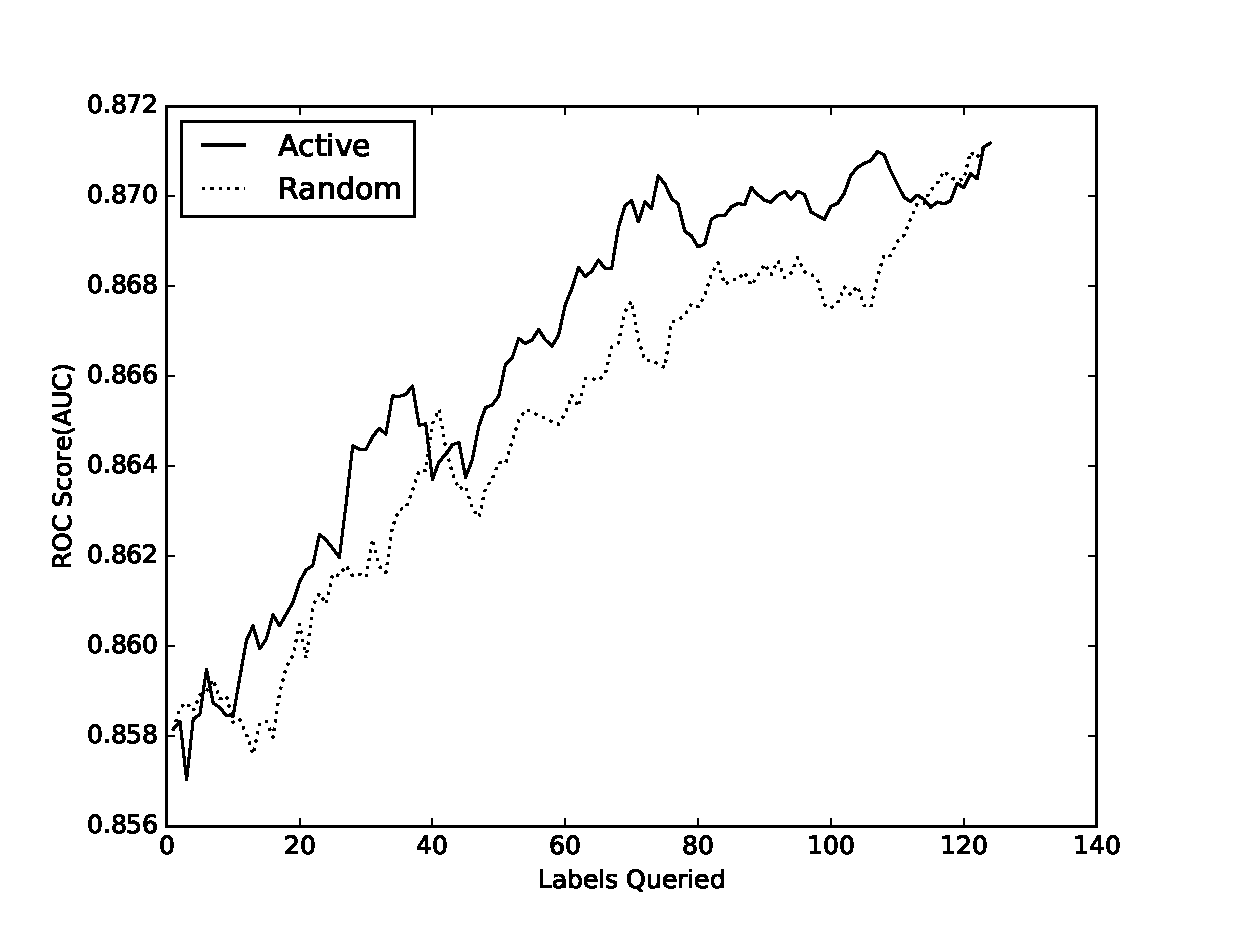
\includegraphics[scale=0.5]{plot}

The above plot shows the increase in ROC score over time as each protein is queried for both the random and active learning methods. Though not by much, the active learner slightly out-paces the baseline. Of course both methods converge to the same ROC score of ~0.87. This is to be expected since at the end both methods have queried all of the proteins and generated the exact same model.   


\section*{Conclusion}
As shown above the active learning method shows slight improvement from the baseline. There are many possible reasons why the improvement was not as significant. Considering these reasons gives insights into future directions that could be taken.

The results seen may be extensively affected by the way the evaluation was performed. The evaluation was unrealistic because all the proteins had the same number of training instances. In a real environment different proteins would have vastly different sizes and as a result different numbers of contained training instances. In the future, evaluation on batches that correctly corresponded to real proteins would be beneficial. 

The size of the query pool could have also negatively affected the evaluation. In a real world scenario the active learner would have access to thousands of DNA-Protein complexes. With a more realistically sized query pool, the divergence between the ROC scores of the active learner and the baseline could possibly be much larger. 

Probably the most important issue with the active learning method, though, is the assumption of linear separability. Because of the noisiness of the labelled data, this assumption is invalid. Because of this, the model cannot use a hard margin and some of the incentives for the scoring method in \cite{active_learning} are somewhat lost. Further work would need to be done in order to handle the loss of separability.

\bibliographystyle{plain}
\bibliography{mybib}{}

\end{document}
